\section{Bluetooth}

Bluetooth is an industrial specification designed for Wireless Personal Area Networks (WPANs). 
It was developed as a low-cost, low-power wireless communication technology. 
The technology was initially conceived as an internal project by Ericsson in 1996-1997, with the goal of creating a universal short-range wireless communication standard.
In 1998, the Bluetooth Special Interest Group (SIG) was formed. 
By 1999, additional industry leaders joined the SIG, further solidifying Bluetooth's position as a global standard.

Bluetooth operates in the ISM 2.4 GHz band and is characterized by its small range, low complexity, and compact size. 
While the original Bluetooth specifications were developed by the industrial consortium, only the first two layers  (PHY and MAC) were later standardized by the IEEE under the 802.15.1 working group.

\subsection{Physical layer}
The physical layer of Bluetooth operates in the globally available ISM band at 2.4 GHz. 
This band is divided into 79 channels (or 23 in countries like France and Japan), each spaced 1 MHz apart, covering the frequency range from 2402 MHz to 2480 MHz. 
The modulation technique used is Gaussian Frequency-Shift Keying (G-FSK).

A key feature of Bluetooth's physical layer is its use of Frequency Hopping Spread Spectrum (FHSS). 
The system hops between frequencies at a rate of 1600 hops per second, with each hop lasting 625 microseconds. 
The hopping sequence is pseudo-random and determined by the clock and address of the "master" device, which regulates channel access.
All other devices in the network, referred to as slaves, follow the hopping sequence defined by the master. 
Packets can be transmitted over durations of 1, 3, or 5 time intervals, depending on the application requirements.

\subsubsection{Piconet}
The simplest network architecture in Bluetooth is called a piconet. 
A piconet is an ad hoc network composed of two or more devices, where one device acts as the master and the others act as slaves. 
Communication within a piconet occurs exclusively between the master and the slaves; direct communication between slaves is not allowed.

A piconet can support up to seven active slaves simultaneously. 
Devices that are part of the piconet but not actively participating in communication can enter a parked state, allowing up to 256 devices to be associated with the piconet in this manner.
Devices not part of the piconet remain in a standby state.

\subsubsection{Architecture}
Bluetooth defines two types of connections to accommodate different communication needs:
\begin{itemize}
    \item \textit{Synchronous Connection-Oriented} (SCO): fixed-rate, bi-directional connection that operates like a circuit-switched link.
        Forward Error Correction (FEC) is used to improve transmission quality.
        The data rate is suitable for voice communication.
    \item \textit{Asynchronous Connection-less} (ACL): packet-switched connection shared between the master and active slaves, based on a polling access scheme.
        Multiple packet formats and physical layer codes are supported, with packets spanning 1, 3, or 5 time slots.
\end{itemize}
\noindent The original Bluetooth protocol architecture did not align with the IEEE 802 structure.
However, it was later adapted by the IEEE to conform to the 802.15.1 specifications. 

\subsubsection{Packets}
Bluetooth packets are structured into three main components, each serving a specific purpose in the communication process:
\begin{itemize}
    \item \textit{Access code}: used for synchronization and piconet identification. 
        It ensures that devices within a piconet can align their frequency hopping sequences and communicate effectively.
        There are three types of access codes: Channel Access Code (CAC), Device Access Code (DAC), and Inquiry Access Code (IAC).
    \item \textit{Header}: contains essential control information for managing the link. 
    \item \textit{Payload}: carries the actual data being transmitted. 
        Its format depends on the type of connection and the packet configuration.
\end{itemize}
\begin{figure}[H]
    \centering
    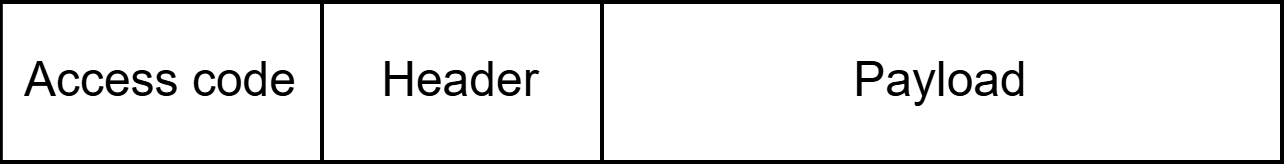
\includegraphics[width=0.5\linewidth]{images/iot19.png}
    \caption{Packet format}
\end{figure}
\noindent Bluetooth devices operate in several states, each corresponding to different phases of communication:
\begin{itemize}
    \item \textit{Stand-by}: the device is inactive, and its radio is powered off to conserve energy.
    \item \textit{Connection}: the device is actively connected to other devices. This state includes sub-states for managing ongoing communication.
    \item \textit{Inquiry}: the device is searching for nearby devices by broadcasting an Inquiry Access Code (IAC).
    \item \textit{Inquiry scan}: the device periodically listens for inquiry requests on specific channels with a low duty cycle.
    \item \textit{Page}: the device attempts to establish a connection with another specific device using the Device Access Code (DAC).
    \item \textit{Page scan}: the device listens for page requests at regular intervals.
\end{itemize}

\begin{figure}[H]
    \centering
    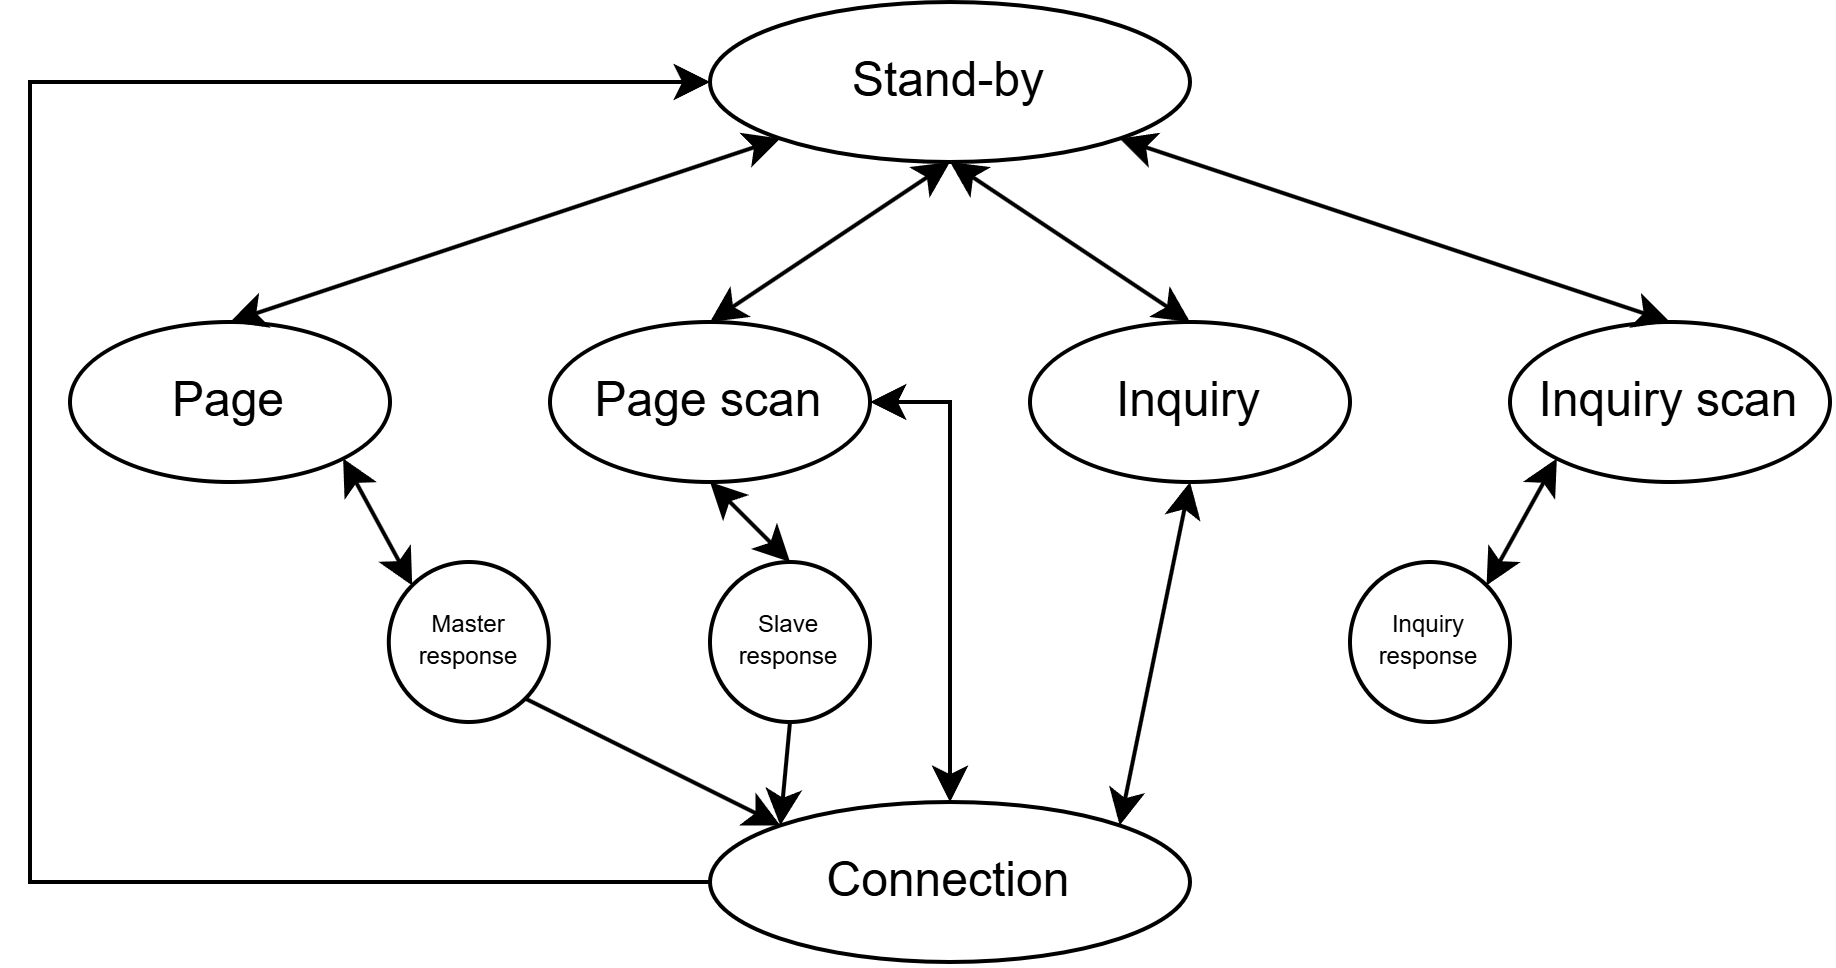
\includegraphics[width=0.5\linewidth]{images/iot20.png}
    \caption{Link controller states}
\end{figure}

\subsection{Profiles}
Bluetooth profiles define basic operation modes tailored to specific applications, ensuring interoperability at the application layer. 
These profiles standardize how devices interact in various use cases, such as audio streaming, file transfer, and hands-free communication. 
By adhering to profiles, manufacturers ensure compatibility across devices from different vendors.

To conserve energy, Bluetooth supports several low-power modes for slave devices in the connection state:
\begin{itemize}
    \item \textit{Hold mode}: the slave temporarily stops listening to the channel for a negotiated period while retaining its AMA. 
        This reduces power consumption without disconnecting the device.
    \item \textit{Sniff mode}: the slave listens to the channel at regular intervals, maintaining its AMA. 
        This mode balances power savings with responsiveness.
    \item \textit{Park mode}: the slave releases its AMA and is assigned a Parked Member Address (PMA). 
        It listens to the channel infrequently (very low duty cycle) and can be reactivated upon receiving an un-park message from the master.
\end{itemize}

\subsection{Bluetooth Low Energy}
Bluetooth Low Energy (BLE) is not intended to replace Bluetooth, but rather coexist alongside it. 
BLE is specifically designed to be energy-efficient, making it ideal for IoT applications.

\subsubsection{Physical layer}
The BLE physical layer operates in the same Industrial, Scientific, and Medical (ISM) band as BR/EDR but with distinct characteristics. 
It uses 40 channels, each 2 MHz wide, with three dedicated to advertisement and broadcast purposes and 37 used for data transfer via adaptive frequency hopping. 
It employs Gaussian Frequency-Shift Keying (GFSK) modulation and supports three PHY types.

\subsubsection{Link layer}
The BLE link layer is governed by a state machine and handles several critical duties. 
It manages different types of packets, supports both public and random addressing schemes, and implements adaptive frequency hopping on the data channels. 
It also manages Asynchronous Connection-Less (ACL) links and ensures reliable communication through sequence numbers (SN) and next expected sequence numbers (NESN) for packet ordering and acknowledgment.

\subsubsection{Features}
Error control in BLE is achieved through sequence numbers and retransmissions. 
Central and peripheral nodes play key roles in BLE communication.
Peripheral nodes periodically transmit advertisements, ranging from 20 milliseconds to 10 seconds, while central nodes scan advertisement channels to detect these broadcasts. 
The central node determines how long to scan (scan window) and how often to perform scans (scan interval).

Adaptive Frequency Hopping (AFH) is a key feature of BLE, where the central node selects channels to avoid interference and shares the channel map with the peripheral node. 

Advertisements in BLE can be directed or undirected, connectable or non-connectable, and scannable or non-scannable. 
Directed advertisements accept connections only from known devices, while undirected ones are open to all. 
Connectable advertisements allow connection establishment, and scannable advertisements permit receiving scan requests and responding accordingly.

A central device can issue a connection request to a peripheral that is broadcasting connectable advertisements. 
The peripheral responds with a connection reply, establishing a connection between the two BLE devices and enabling them to exchange data. 
Once connected, the two devices use the Attribute Protocol (ATT) for data exchange. 
In this protocol, the client can discover available attributes or resources on the server and perform read and write operations on these attributes.